\chapter{Interaksi Antarspesies}\label{ch:b1:species-interactions}

Pada 1963, di sebuah pantai berbatu di Pasifik, seorang ahli ekologi
muda mulai melemparkan tiap bintang laut yang ditemukannya pada
sepetak batu kembali ke lautnya, lalu terus melakukannya
bertahun-tahun. Bintang lautnya memakan kerang biru. Tanpa bintang
lautnya, kerang birunya menyebar turun pada batunya lalu menyesaki
teritip, siput topi, kiton dan alga yang tadinya hidup di situ; sebuah
\omterm{def:b1:ecosystem-organization:ecosystem}{komunitas} lima belas spesies jatuh menjadi delapan. Satu pemangsa,
yang sendirinya tidak melimpah maupun besar, telah menahan seluruh
himpunannya di tempatnya. Spesies tidak sekadar berbagi sebuah tempat;
keduanya bersaing memperebutkannya, saling memakan, hidup di dalam dan
di atas satu sama lain, serta saling bergantung, dan \omterm{def:b1:ecosystem-organization:ecosystem}{komunitasnya}
adalah jumlah interaksi ini. Bab ini menggolongkannya, memberikan
model kuantitatif \omterm{def:b1:species-interactions:types}{persaingan} dan \omterm{def:b1:species-interactions:types}{pemangsaan} yang sanggup ditangani
tahun pertama, lalu memperlihatkan lewat percobaan bagaimana satu
interaksi dapat membentuk sebuah \omterm{def:b1:ecosystem-organization:ecosystem}{ekosistem} utuh.

\section{Sebuah penggolongan interaksi}

\begin{definition}[Interaksi antarspesies]\label{def:b1:species-interactions:types}
\index{persaingan}\index{pemangsaan}\index{parasitisme}\index{mutualisme}\index{komensalisme}
Sebuah interaksi antara dua spesies digolongkan menurut pengaruhnya
pada masing-masing: $+$ (untung), $-$ (rugi) atau $0$.
\emph{Persaingan} ($-/-$): keduanya memakai sebuah sumber daya yang
pasokannya kurang. \emph{Pemangsaan} ($+/-$): yang satu membunuh lalu
memakan yang lain; \emph{herbivori} ($+/-$) ketika yang dimakan adalah
sebatang tumbuhan dan biasanya sintas; \emph{parasitisme} ($+/-$)
ketika pengeksploitasinya hidup pada atau dalam seekor inang yang tidak
dibunuhnya segera. \emph{Mutualisme} ($+/+$): keduanya untung.
\emph{Komensalisme} ($+/0$): yang satu untung, yang lain tak
terpengaruh. \emph{Amensalisme} ($-/0$): yang satu rugi, yang lain tak
terpengaruh. Tiap interaksinya adalah sebuah tekanan pemilihan atas
kedua sekutunya, dan penyesuaian timbal baliknya sepanjang generasi
adalah \emph{koevolusi}.
\end{definition}

\begin{example}[Satu pohon, keenamnya]\label{ex:b1:species-interactions:oak}
Sebatang pohon ek bersaing dengan tetangganya memperebutkan cahaya;
bijinya dimakan burung jay (\omterm{def:b1:species-interactions:types}{pemangsaan}) dan \omterm{def:b1:flowering-plant-organization:organs}{daunnya} dimakan ulat
(herbivori); benalu menarik getahnya (\omterm{def:b1:species-interactions:types}{parasitisme}); \omterm{def:b1:flowering-plant-organization:organs}{akarnya} menukar
gula dengan fosfat bersama sebuah jamur (\omterm{def:b1:species-interactions:types}{mutualisme}); paku-pakuan
tumbuh pada kulit kayunya, yang dipakainya hanya sebagai tempat
bertengger (\omterm{def:b1:species-interactions:types}{komensalisme}); dan naungannya membunuh rumput di bawahnya
(amensalisme).
\end{example}

\section{Persaingan}

\begin{definition}[Persaingan antarspesies]\label{def:b1:species-interactions:competition}
\index{penyisihan bersaing}\index{pembagian relung}\index{pergeseran ciri}
Dua spesies bersaing ketika keduanya memakai sebuah sumber daya ---
makanan, cahaya, air, ruang, tempat bersarang --- yang pasokannya
membatasi pertumbuhannya. \omterm{def:b1:species-interactions:types}{Persaingannya} dapat berupa
\emph{eksploitasi} (masing-masing mengambil apa yang akan dipakai yang
lain) atau \emph{gangguan} (keagresifan langsung, toksin, teritori).
Hasilnya mengikuti \emph{asas penyisihan bersaing}: dua spesies yang
memerlukan sumber daya pembatas yang sama dengan cara yang sama tak
dapat hidup berdampingan tanpa batas dalam sebuah \omterm{def:b1:organism-environment:organism}{lingkungan} yang
tetap; pesaing yang lebih baik meniadakan yang lain. Karena itu
pesaing yang berdampingan berbeda \omterm{def:b1:ecosystem-organization:niche}{relungnya} (\emph{pembagian \omterm{def:b1:ecosystem-organization:niche}{relung}})
--- dan tempat dua spesies bertumpang tindih keduanya sering menyimpang
dalam bentuk lebih daripada tempat masing-masing hidup sendirian
(\emph{pergeseran ciri}).
\end{definition}

\begin{proposition}[Model persaingan Lotka--Volterra]\label{prop:b1:species-interactions:lotka}
Biarkan dua spesies tumbuh secara logistik (\cref{ch:b1:populations})
dan biarkan tiap individu spesies 2 terhitung sebagai $\alpha$ individu
spesies 1 dalam pemakaian sumber daya spesies 1, dan tiap individu
spesies 1 sebagai $\beta$ individu spesies 2:
\[
\frac{\dd N_1}{\dd t} = r_1 N_1\left(1 - \frac{N_1 + \alpha N_2}{K_1}\right),
\qquad
\frac{\dd N_2}{\dd t} = r_2 N_2\left(1 - \frac{N_2 + \beta N_1}{K_2}\right).
\]
Spesies 1 berhenti tumbuh pada garis $N_1 + \alpha N_2 = K_1$
(\emph{isoklin}\index{isoklin}nya), spesies 2 pada $N_2 + \beta N_1 = K_2$. Bila
tiap spesiesnya membatasi dirinya lebih daripada ia membatasi yang lain ($\alpha <
K_1/K_2$ dan $\beta < K_2/K_1$) \omterm{prop:b1:species-interactions:lotka}{isoklinnya} berpotongan dengan
kesetimbangan kedua spesiesnya mantap dan keduanya \emph{berdampingan};
bila satu \omterm{prop:b1:species-interactions:lotka}{isoklinnya} terletak seluruhnya di atas yang lain, spesies itu
selalu \emph{menyisihkan} yang lain; bila masing-masing membatasi yang
lain lebih daripada dirinya, pemenangnya bergantung pada jumlah awalnya.
\end{proposition}
\begin{proof}[Bukti sebagian]
Spesies 1 tumbuh di bawah \omterm{prop:b1:species-interactions:lotka}{isoklinnya} lalu menyusut di atasnya; spesies
2 demikian juga. Ketika \omterm{prop:b1:species-interactions:lotka}{isoklinnya} berpotongan dengan \omterm{prop:b1:species-interactions:lotka}{isoklin} spesies
1 di atas \omterm{prop:b1:species-interactions:lotka}{isoklin} spesies 2 pada sumbu $N_1$ dan di bawahnya pada
sumbu $N_2$, sebuah titik di luar perpotongannya didorong kembali
menujunya dari tiap sisinya: perpotongannya adalah sebuah kesetimbangan
mantap dengan kedua spesiesnya hadir. Ketika \omterm{prop:b1:species-interactions:lotka}{isoklin} spesies 1
terletak seluruhnya di luar \omterm{prop:b1:species-interactions:lotka}{isoklin} spesies 2, tiap titik tempat
spesies 2 masih dapat tumbuh juga sebuah titik tempat spesies 1 tumbuh
dan ia terus tumbuh sesudah spesies 2 berhenti, sampai ia mencapai
$K_1$ dengan $N_2 = 0$. Telaah penuhnya dikerjakan dalam jilid Tahun
ke-2; sketsa \omterm{prop:b1:species-interactions:lotka}{isoklinnya} memberikan tiap hasilnya tanpa itu.
\end{proof}

\begin{omfigure}
\begin{tikzpicture}[font=\footnotesize, >=Stealth, line cap=round]
  \begin{scope}
    \draw[->, thick] (0,0) -- (4.6,0) node[below left] {$N_1$};
    \draw[->, thick] (0,0) -- (0,4.4) node[below right] {$N_2$};
    \draw[very thick, omDef] (4.0,0) -- (0,3.0) node[pos=0.15, above right, omDef!80!black] {spesies 1 berhenti};
    \draw[very thick, omThm] (2.6,0) -- (0,4.0) node[pos=0.85, right, omThm!80!black] {spesies 2 berhenti};
    \fill (1.63,1.78) circle (2pt); \node[anchor=west] at (1.75,1.95) {berdampingan mantap};
    \draw[->, gray] (3.6,3.0) -- (2.2,2.2); \draw[->, gray] (0.4,0.4) -- (1.3,1.4);
    \node[anchor=north] at (2.3,-0.8) {tiap spesies membatasi dirinya lebih};
  \end{scope}
  \begin{scope}[xshift=7.2cm]
    \draw[->, thick] (0,0) -- (4.6,0) node[below left] {$N_1$};
    \draw[->, thick] (0,0) -- (0,4.4) node[below right] {$N_2$};
    \draw[very thick, omDef] (4.0,0) -- (0,4.0) node[pos=0.5, above right, omDef!80!black] {spesies 1 berhenti};
    \draw[very thick, omThm] (2.4,0) -- (0,2.4) node[pos=0.35, anchor=north east, align=right, omThm!80!black] {spesies 2\\ berhenti};
    \fill (4.0,0) circle (2pt); \node[anchor=north, font=\scriptsize] at (3.5,-0.3) {spesies 1 sendirian pada $K_1$};
    \draw[->, gray] (1.0,3.4) -- (2.1,2.3); \draw[->, gray] (2.4,2.0) -- (3.4,0.7);
    \node[anchor=north] at (2.3,-0.8) {spesies 1 menang di mana-mana};
  \end{scope}
\end{tikzpicture}

{\small Dua hasil \omterm{def:b1:species-interactions:types}{persaingan} dua spesies, yang dibaca dari \omterm{prop:b1:species-interactions:lotka}{isoklinnya}
(garis tempat tiap spesiesnya berhenti tumbuh). Kiri: \omterm{prop:b1:species-interactions:lotka}{isoklinnya}
berpotongan sehingga tiap spesiesnya ditahan lebih oleh dirinya
daripada oleh yang lain, dan keduanya berdampingan. Kanan: \omterm{prop:b1:species-interactions:lotka}{isoklin}
spesies 1 terletak di luar \omterm{prop:b1:species-interactions:lotka}{isoklin} spesies 2, dan spesies 1 selalu
menang.}
\end{omfigure}

\begin{proposition}[Penyisihan bersaing]\label{prop:b1:species-interactions:gause}
\index{asas Gause}
Dua spesies yang bersaing memperebutkan satu sumber daya pembatas
dalam sebuah \omterm{def:b1:organism-environment:organism}{lingkungan} yang tetap tak dapat bertahan berdua: yang
\omterm{def:b1:populations:population}{populasinya} sanggup terus tumbuh pada aras sumber daya yang lebih
rendah menyeret sumber dayanya di bawah apa yang diperlukan yang lain,
dan yang lain menyusut sampai punah.
\end{proposition}
\begin{proof}[Bukti]
Gause (1934) menumbuhkan dua siliata, \emph{Paramecium aurelia} dan
\emph{P.~caudatum}, pada sebuah ransum bakteri harian. Sendirian,
masing-masing tumbuh secara logistik sampai datarannya sendiri.
Bersama, \emph{P.~aurelia}, yang tumbuh lebih cepat dan memerlukan
lebih sedikit makanan tiap individu, mencapai nyaris datarannya
sedangkan \emph{P.~caudatum} menyusut menjadi nol dalam enam belas
hari. Sebuah spesies ketiga, \emph{P.~bursaria}, yang makan di dasar
tabungnya tempat \emph{P.~aurelia} tidak, berdampingan dengannya tanpa
batas: penyisihannya berlaku hanya ketika \omterm{def:b1:ecosystem-organization:niche}{relungnya} sama.
\end{proof}

\begin{omfigure}
\begin{tikzpicture}
\begin{axis}[
  width=0.8\linewidth, height=6.2cm,
  axis x line=bottom, axis y line=left,
  xmin=0, xmax=20, ymin=0, ymax=220,
  xlabel={hari}, ylabel={individu tiap \qty{0.5}{mL}},
  xlabel style={font=\small}, ylabel style={font=\small},
  tick label style={font=\small},
  legend style={font=\scriptsize, at={(0.98,0.02)}, anchor=south east, draw=none, fill=none},
  legend cell align=left,
]
\addplot[omDef, very thick, dashed, domain=0:20, samples=60] {200/(1+40*exp(-0.8*x))};
\addlegendentry{\emph{P.~aurelia} sendirian}
\addplot[omThm, very thick, dashed, domain=0:20, samples=60] {130/(1+25*exp(-0.55*x))};
\addlegendentry{\emph{P.~caudatum} sendirian}
\addplot[omDef, very thick, domain=0:20, samples=60] {170/(1+40*exp(-0.65*x))};
\addlegendentry{\emph{P.~aurelia} tercampur}
\addplot[omThm, very thick, domain=0:20, samples=80] {80*exp(-0.05*(x-6)^2)*(x<12) + 80*exp(-0.05*36)*exp(-0.5*(x-12))*(x>=12)};
\addlegendentry{\emph{P.~caudatum} tercampur}
\end{axis}
\end{tikzpicture}

{\small Percobaan \omterm{def:b1:species-interactions:types}{persaingan} Gause (digambar ulang dari datanya). Tiap
spesiesnya sendirian tumbuh sampai datarannya; bersama,
\emph{P.~aurelia} naik nyaris sampai datarannya sendiri sedangkan
\emph{P.~caudatum} memuncak lalu diseret sampai punah.}
\end{omfigure}

\begin{example}[Pergeseran ciri pada burung pipit]\label{ex:b1:species-interactions:finches}
Di pulau tempat satu jenis burung pipit tanah hidup sendirian
paruhnya berukuran tengah; tempat dua spesies berbagi sebuah pulau
paruhnya masing-masing lebih kecil dan lebih besar daripada yang
dimiliki masing-masing sendirian, tiap spesiesnya telah bergeser
menuju biji yang tak sanggup dipecahkan yang lain. \omterm{def:b1:ecosystem-organization:niche}{Relungnya} dibagi
oleh evolusinya, dan pembagiannya terlihat pada paruhnya.
\end{example}

\section{Pemangsaan dan herbivori}

\begin{definition}[Tanggapan fungsional]\label{def:b1:species-interactions:functional}
\index{tanggapan fungsional}\index{waktu penanganan}
Yang disebut \emph{tanggapan fungsional} seekor pemangsa adalah cacah
mangsa yang dimakan satu pemangsa tiap satuan waktu sebagai sebuah
fungsi kerapatan mangsanya $N$. \emph{Jenis I}: sebanding dengan $N$
(seekor pemakan saring). \emph{Jenis II}: naik lalu menjenuh, sebab
tiap mangsanya memakan sebuah \emph{waktu penanganan} $h$ untuk
ditangkap, dimakan dan dicerna, yang selama itu tak ada yang lain
dapat diambil. \emph{Jenis III}: sigmoid --- rendah pada kerapatan
rendah sebab pemangsanya mengabaikan atau tak sanggup menemukan mangsa
yang jarang, lalu naik curam (seekor pemangsa yang beralih ke apa pun
yang lazim). Yang disebut \emph{tanggapan numerik} adalah perubahan
cacah pemangsanya bersama kerapatan mangsanya, lewat pembiakan atau
imigrasi.
\end{definition}

\begin{theorem}[Persamaan cakram]\label{thm:b1:species-interactions:holling}
\index{persamaan cakram}
Bila seekor pemangsa mencari pada sebuah \emph{laju serangan} $a$
(luas yang disapu tiap satuan waktu, dikali peluang penangkapannya)
lalu membelanjakan sebuah \omterm{def:b1:species-interactions:functional}{waktu penanganan} $h$ pada tiap mangsanya,
cacah mangsa yang diambil tiap pemangsa tiap satuan waktu pada
kerapatan mangsa $N$ adalah
\[
f(N) = \frac{aN}{1 + ahN} ,
\]
yang naik linear sebagai $aN$ pada kerapatan rendah lalu menjenuh pada
$1/h$ pada kerapatan tinggi; $f$ bernilai separuh maksimumnya ketika
$N = 1/(ah)$. Dalam bentuk $1/f = 1/(aN) + h$ sebuah gambar $1/f$
terhadap $1/N$ adalah sebuah garis lurus berkemiringan $1/a$ dengan
potongan $h$.
\end{theorem}
\begin{proof}
Sepanjang sebuah waktu total $T$ pemangsanya mencari selama $T_s$ lalu
menangani selama sisanya. Ketika mencari, ia berjumpa mangsa pada laju
$aN$, sehingga cacah yang tertangkap adalah $n = aN T_s$; menanganinya
memakan $nh$, sehingga $T = T_s + nh =
n/(aN) + nh$, dari situ $n/T = aN/(1 + ahN)$. Ketika $ahN \ll 1$
penanganannya dapat diabaikan dan $f \approx aN$; ketika $ahN \gg 1$
pemangsanya tak berbuat apa pun selain menangani dan $f \to 1/h$.
Membalikkannya memberi bentuk linearnya.
\end{proof}
\begin{proof}[Bukti]
Holling (1959) menyuruh seorang pembantu bermata tertutup ``memangsa''
dengan sebuah ujung jari pada cakram amplas yang ditaburkan di sebuah
meja, sambil memungut tiap cakram yang ditemukannya (\omterm{def:b1:species-interactions:functional}{waktu
penanganannya}) sebelum mencari lagi; cacah yang ditemukan tiap menit
terhadap kerapatan cakramnya memberikan tepat kurva ini, dan
persamaannya mengambil namanya dari percobaannya. Pemangsa nyata ---
seekor belalang sembah pada lalat, seekor ikan berduri pada kutu air
--- memberi bentuk yang sama, dengan \omterm{def:b1:species-interactions:functional}{waktu penanganan} beberapa sekon
sampai beberapa jam.
\end{proof}

\begin{omfigure}
\begin{tikzpicture}
\begin{axis}[
  width=0.78\linewidth, height=6.2cm,
  axis x line=bottom, axis y line=left,
  xmin=0, xmax=100, ymin=0, ymax=12,
  xlabel={kerapatan mangsa $N$ (tiap \unit{m^2})}, ylabel={mangsa yang dimakan tiap pemangsa tiap hari},
  xlabel style={font=\small}, ylabel style={font=\small},
  tick label style={font=\small},
  legend style={font=\scriptsize, at={(0.98,0.03)}, anchor=south east, draw=none, fill=none},
  legend cell align=left,
]
\addplot[omExo!80!black, very thick, domain=0:100, samples=2] {0.1*x};
\addlegendentry{jenis I: $f = aN$}
\addplot[omDef, very thick, domain=0:100, samples=80] {0.5*x/(1+0.05*x)};
\addlegendentry{jenis II: $f = aN/(1+ahN)$, dataran $1/h = 10$}
\addplot[omThm, very thick, domain=0:100, samples=80] {10*x^2/(30^2+x^2)};
\addlegendentry{jenis III: sigmoid}
\draw[dashed, gray] (axis cs:0,10) -- (axis cs:100,10);
\end{axis}
\end{tikzpicture}

{\small Ketiga \omterm{def:b1:species-interactions:functional}{tanggapan fungsionalnya}. Jenis II menjenuh pada $1/h$
(di sini sepuluh mangsa sehari, sebuah \omterm{def:b1:species-interactions:functional}{waktu penanganan}
\qty{2.4}{h}); jenis III mulai perlahan sebab mangsa yang jarang
terlewatkan.}
\end{omfigure}

\begin{proposition}[Pertahanan dan lomba senjata]\label{prop:b1:species-interactions:defences}
\index{mimikri}\index{aposematisme}
Mangsa dan tumbuhan mengembangkan pertahanan --- kripsis, baju zirah,
duri, kecepatan, toksin dan warna peringatannya (\emph{aposematisme}),
serta \emph{mimikri}: sebuah spesies tak berbahaya yang meniru sebuah
spesies beracun (Batesian) atau beberapa spesies beracun yang memusat
pada satu pola (Müllerian). Tumbuhan mempertahankan dirinya dengan
duri, silika, tanin, alkaloid dan glikosida sianogenik, yang sering
diimbas kerusakannya. Pemangsa dan herbivora mengembangkan lawan
tindakan --- indra yang lebih tajam, \omterm{def:b1:enzymes:enzyme}{enzim} penawar racun, ketahanan
terhadap toksinnya --- dan pasangannya berkoevolusi. Hasilnya bukanlah
kemusnahan mangsanya melainkan sebuah neraca yang berjalan: seekor
pemangsa yang memakan mangsanya sampai punah akan menyusulnya.
\end{proposition}

\begin{omfigure}
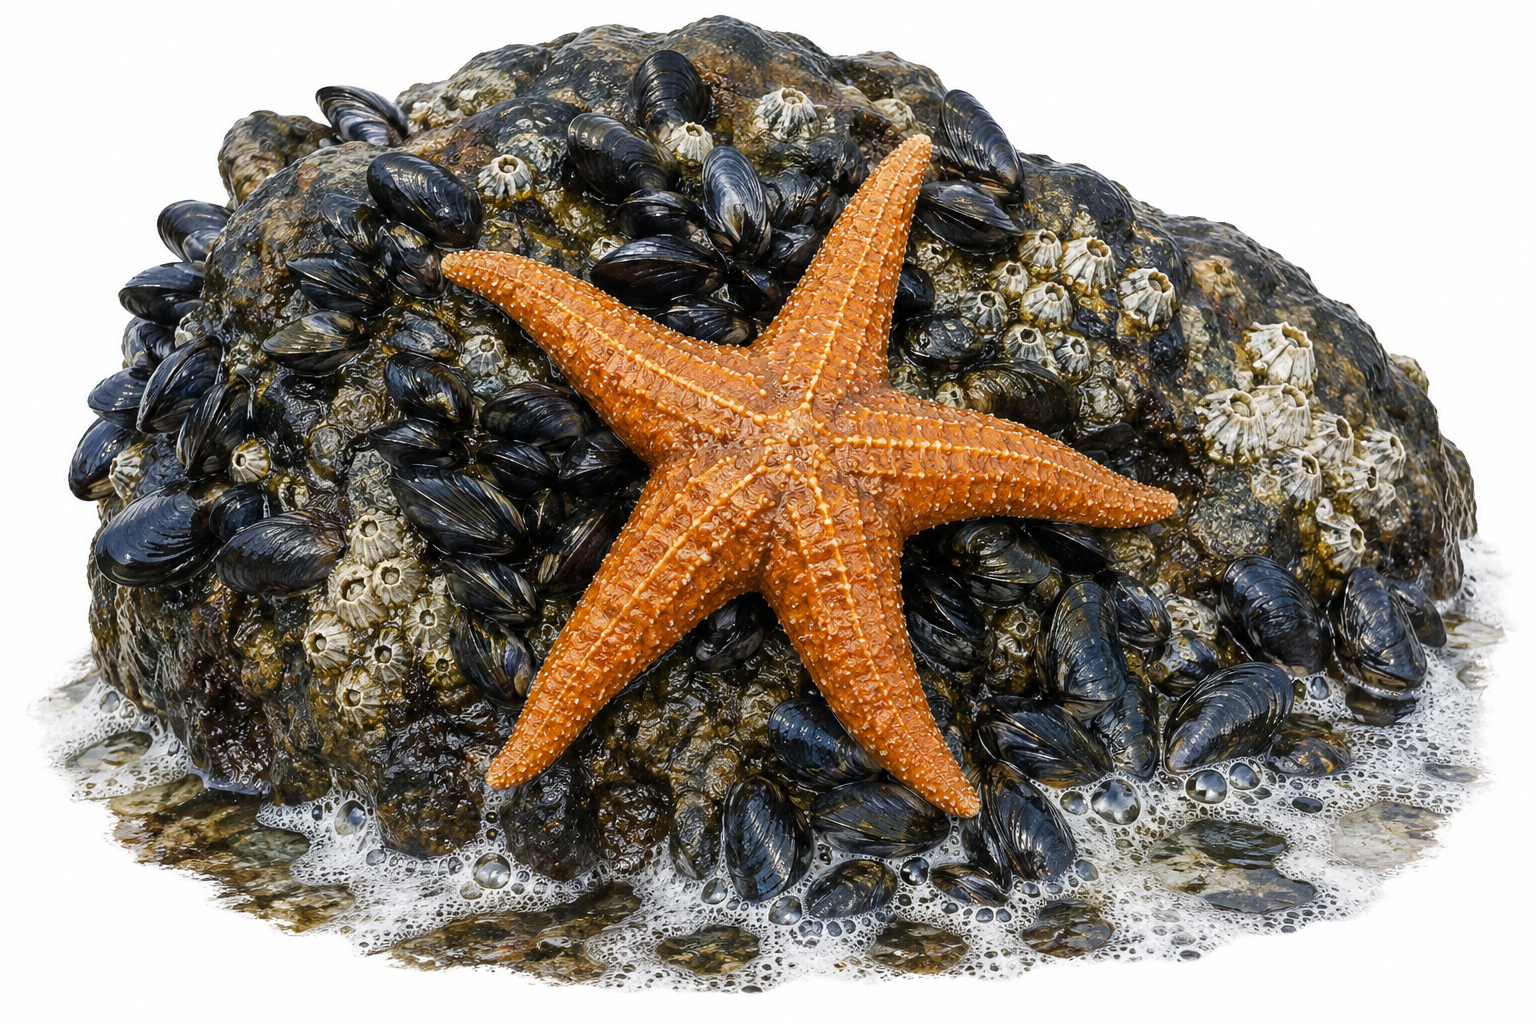
\includegraphics[width=0.6\linewidth]{images/book3/ai/b3-27-sea-star-mussels.png}

{\small Seekor bintang laut pemangsa pada sebuah hamparan kerang biru
pada surut: pemangsa kunci yang penyingkirannya mengubah sebuah pantai
lima belas spesies menjadi sebuah monokultur kerang biru.}
\end{omfigure}

\section{Hidup bersama: parasitisme, mutualisme, komensalisme}

\begin{definition}[Parasitisme, simbiosis, mutualisme]\label{def:b1:species-interactions:symbiosis}
\index{simbiosis}\index{parasit}\index{lumut kerak}
Seekor \emph{parasit} hidup atas beban seekor inang, pada tubuhnya
(ektoparasit: caplak, kutu, benalu) atau di dalamnya (endoparasit:
cacing pita, parasit malaria, jamur karat), sambil mengambil zat gizi
lalu menurunkan kebugarannya tanpa mesti membunuhnya; parasit sering
mengkhusus, dengan daur hidup rumit yang melewati beberapa inang.
Sebuah \emph{simbiosis} adalah persekutuan yang erat dan bertahan lama
antara dua spesies mana pun; sebuah \emph{\omterm{def:b1:species-interactions:types}{mutualisme}} adalah yang
menguntungkan keduanya: \omterm{def:b1:plant-water-minerals:mycorrhiza}{mikorizanya} (sebuah jamur pada atau dalam \omterm{def:b1:flowering-plant-organization:organs}{akar}
tumbuhan, yang menukar fosfat dan air dengan gula;
\cref{ch:b1:plant-water-minerals}), \omterm{def:b1:plant-water-minerals:nodules}{bintil akarnya} (bakteri
pemancang nitrogen yang diberi makan legumnya), \emph{lumut kerak}
(sebuah jamur yang memondokkan sebuah alga atau sianobakterium), karang
terumbunya (seekor knidaria yang memondokkan dinoflagelata
berfotosintesis), mikrobiota usus seekor ruminansia atau seekor rayap
(\cref{ch:b1:digestion-absorption}), dan penyerbukannya (nektar
ditukar dengan pengangkutan serbuk sarinya). Banyak \omterm{def:b1:species-interactions:types}{mutualisme} bermula
sebagai \omterm{def:b1:species-interactions:types}{parasitisme} atau \omterm{def:b1:species-interactions:types}{pemangsaan} yang koevolusi sekutunya ubah
menjadi keuntungan bersama, dan tetap bersyarat: sebuah jamur \omterm{def:b1:plant-water-minerals:mycorrhiza}{mikoriza}
dalam tanah yang kaya fosfat menjadi sebuah biaya, dan tumbuhannya
menguranginya.
\end{definition}

\begin{example}[Penyerbukan sebagai sebuah dagangan]\label{ex:b1:species-interactions:pollination}
Sekuntum bunga membelanjakan beberapa joule gula pada nektarnya;
seekor lebah membelanjakan penerbangan untuk mengumpulkannya lalu
membawa serbuk sari antarbunga seraya pergi. Warna, harum, bentuk dan
waktu bunganya ditujukan kepada penyerbuknya, dan panjang lidah,
penglihatan warna serta ingatan mencari makan lebahnya kepada
bunganya; sebagian pasangannya begitu rapat terpasangkan --- sebuah
taji nektar yang panjang dan satu ngengat yang lidahnya mencapainya
--- sehingga tak satu pun sintas tanpa yang lain, dan sebuah \omterm{def:b1:ecosystem-organization:ecosystem}{komunitas}
tumbuhan utuh dapat bergantung pada beberapa spesies serangga.
\end{example}

\begin{omfigure}
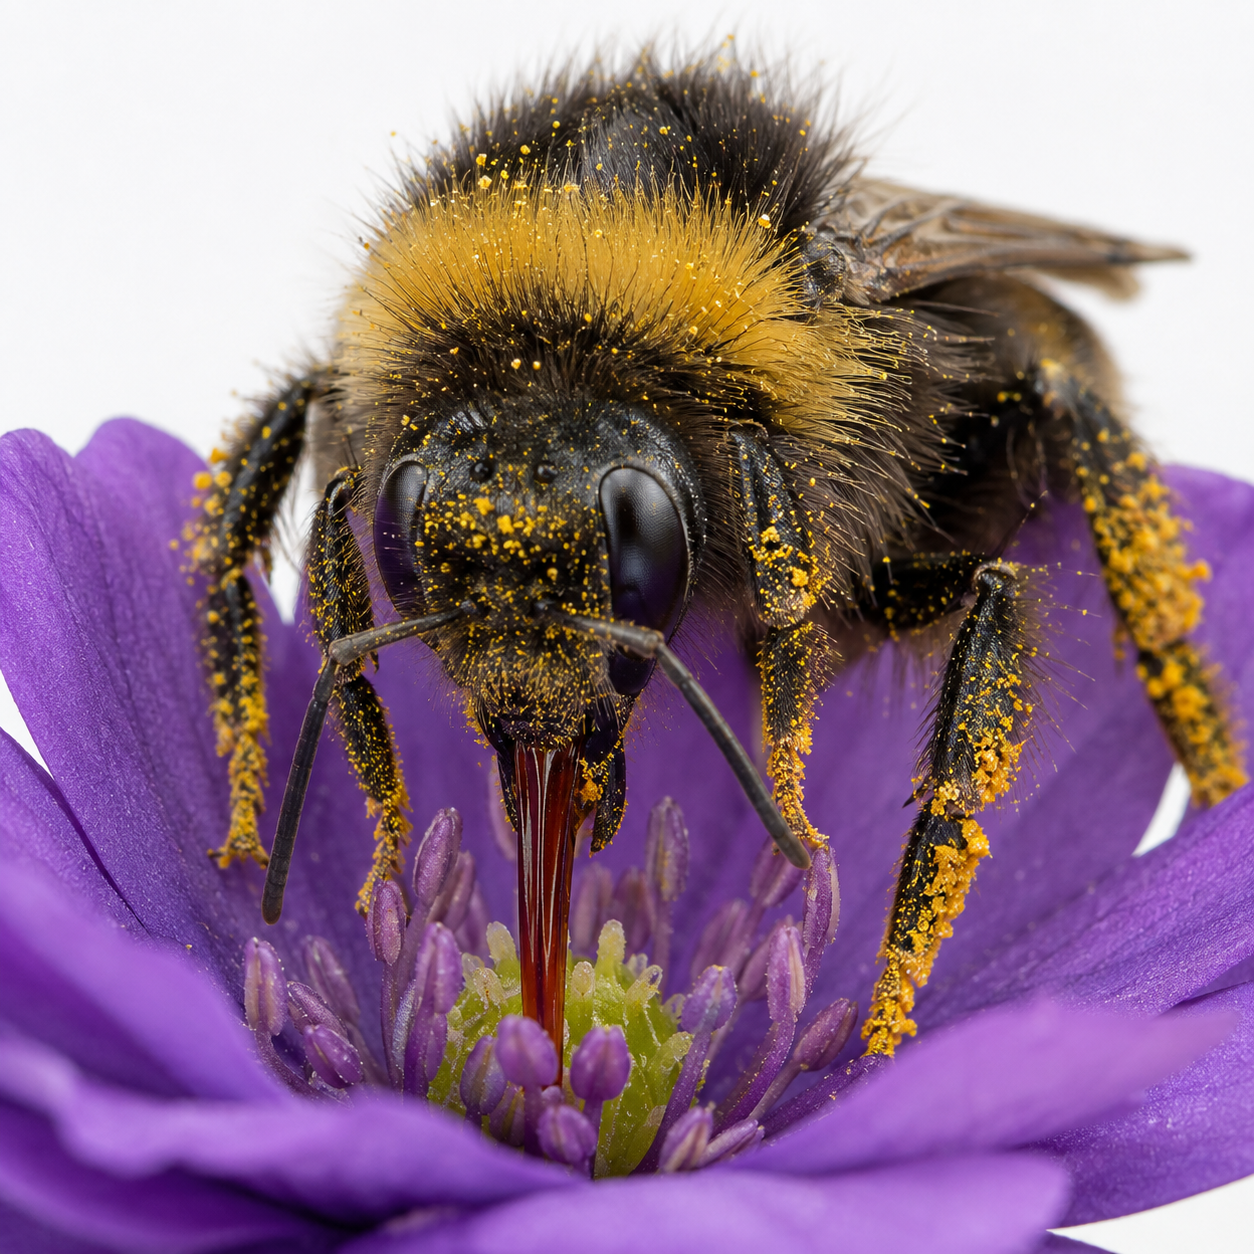
\includegraphics[width=0.56\linewidth]{images/book3/ai/b3-27-bee-flower.png}

{\small Sebuah \omterm{def:b1:species-interactions:types}{mutualisme} yang bekerja: nektar bagi lebahnya,
pengangkutan serbuk sari bagi bunganya. Bentuk tiap sekutunya telah
dibentuk yang lain.}
\end{omfigure}

\begin{remark}[Komensalisme itu jarang dan tak mantap]\label{rem:b1:species-interactions:commensal}
Sedikit interaksi yang benar-benar $+/0$: epifit yang menaungi
inangnya, remora yang memakan biaya seret sedikit pada hiunya, kuntul
kerbau yang memakan apa yang diaduk kerbaunya hanyalah komensal sejauh
ketelitian pengukurannya. Interaksi digolongkan menurut pengaruh
bersihnya, dan pengaruh bersihnya dapat berubah bersama keadaannya.
\end{remark}

\section{Interaksi yang membentuk komunitasnya}

\begin{definition}[Spesies kunci, riam trofik]\label{def:b1:species-interactions:keystone}
\index{spesies kunci}\index{riam trofik}
Yang disebut \emph{spesies kunci} adalah spesies yang pengaruhnya pada
\omterm{def:b1:ecosystem-organization:ecosystem}{komunitasnya} tidak sebanding dengan kelimpahan atau biomassanya:
singkirkanlah ia dan struktur \omterm{def:b1:ecosystem-organization:ecosystem}{komunitasnya} berubah, biasanya sebab ia
mengendalikan sebuah pesaing yang mendominasi. Yang disebut
\emph{riam trofik} adalah perambatan sebuah pengaruh menuruni sebuah
\omterm{def:b1:ecosystem-organization:foodweb}{rantai makanan} melintasi lebih dari satu aras: hadirnya seekor
pemangsa menurunkan herbivoranya, yang menaikkan tumbuhannya;
penyingkirannya berbuat sebaliknya. Riamnya memperlihatkan bahwa
\omterm{def:b1:ecosystem-organization:ecosystem}{komunitas} terstruktur dari atas maupun dari bawah (oleh
produktivitasnya, \cref{ch:b1:ecosystem-organization}).
\end{definition}

\begin{proposition}[Seekor pemangsa dapat memelihara keanekaragaman]\label{prop:b1:species-interactions:paine}
Dengan memakan spesies yang bila tidak akan memenangi \omterm{def:b1:species-interactions:types}{persaingan}
memperebutkan ruang atau sumber daya, seekor pemangsa memelihara yang
kalah dalam \omterm{def:b1:ecosystem-organization:ecosystem}{komunitasnya}; penyingkirannya membiarkan pesaing yang
mendominasi menyisihkannya, dan keanekaragamannya turun.
\end{proposition}
\begin{proof}[Bukti]
Paine (1966) menyingkirkan bintang laut \emph{Pisaster} dari sepetak
pantai berbatu sepanjang \qty{8}{m} di pesisir Pasifik Amerika Utara
lalu meninggalkan sepetak tetangganya sebagai kendali. Bintang lautnya
memakan kerang biru, teritip dan hewan menetap lainnya, dengan kerang
biru sebagai pilihan utamanya. Dalam dua tahun kerang biru
\emph{Mytilus} telah menyebar menuruni batunya lalu mengambil hampir
seluruh ruangnya; teritip, kiton, siput topi dan alga yang tadinya
hidup dalam celahnya lenyap, dan lima belas spesies petak kendalinya
jatuh menjadi delapan. Bagian pemangsanya sendiri dari biomassa
\omterm{def:b1:ecosystem-organization:ecosystem}{komunitasnya} kecil; penyingkirannya mengubah segalanya.
\end{proof}

\begin{omfigure}
\begin{tikzpicture}
\begin{axis}[
  width=0.74\linewidth, height=5.6cm,
  axis x line=bottom, axis y line=left,
  xmin=1963, xmax=1969, ymin=0, ymax=18,
  xlabel={tahun}, ylabel={spesies pada petaknya},
  xlabel style={font=\small}, ylabel style={font=\small},
  tick label style={font=\small}, xtick={1963,1964,1965,1966,1967,1968},
  x tick label style={/pgf/number format/1000 sep=},
  legend style={font=\scriptsize, at={(0.98,0.03)}, anchor=south east, draw=none, fill=none},
  legend cell align=left,
]
\addplot[omDef, very thick, mark=*] coordinates {(1963,15) (1964,15) (1965,14) (1966,15) (1967,15) (1968,15)};
\addlegendentry{kendali: bintang lautnya hadir}
\addplot[omThm, very thick, mark=square*] coordinates {(1963,15) (1964,12) (1965,10) (1966,9) (1967,8) (1968,8)};
\addlegendentry{bintang lautnya disingkirkan}
\node[font=\scriptsize, anchor=south west, align=left] at (axis cs:1966.2,10.6) {kerang birunya mengambil\\ batunya};
\end{axis}
\end{tikzpicture}

{\small Percobaan penyingkiran Paine (menurut datanya). Keanekaragaman
pada petak tanpa pemangsanya turun separuh dalam lima tahun sedangkan
kendalinya memegang lima belas spesiesnya.}
\end{omfigure}

\begin{example}[Serigala, rusa elk dan pohon dedalu]\label{ex:b1:species-interactions:wolves}
Serigala dimusnahkan dari sebuah taman pegunungan yang luas pada
1920-an; rusa elknya berlipat ganda lalu merambah pohon dedalu dan
aspen di sepanjang sungainya sampai menjadi tunggul; berang-berang,
yang memerlukan dedalu, menyusut; burung penyanyi kehilangan semak
belukarnya. Ketika serigalanya dimasukkan kembali pada 1995 rusa
elknya menyusut dan, yang lebih penting, menghindari dasar lembah
tempat keduanya rentan; dedalunya tumbuh kembali, berang-berangnya
kembali lalu membangun bendungan, dan lahan basah yang dibuatnya
membawa kembali ikan, amfibia dan burung. Riamnya berjalan dari
seekor karnivora lewat seekor herbivora ke tumbuhannya lalu dari situ
ke selusin spesies yang tak pernah bertemu seekor serigala --- dengan
cuaca, perburuan dan pemangsa lain menyumbang, sehingga bagian
serigalanya dalam perubahannya masih diperdebatkan.
\end{example}

\begin{omfigure}
\begin{tikzpicture}[font=\footnotesize, >=Stealth, line cap=round,
  lv/.style={draw, thick, rounded corners=3pt, inner sep=4pt, align=center, fill=white, minimum width=2.6cm}]
  \node[lv, fill=omDef!25] (wolf) at (0,4.5) {serigala};
  \node[lv, fill=omProp!20] (elk) at (0,2.8) {rusa elk};
  \node[lv, fill=omExo!20] (willow) at (0,1.1) {dedalu, aspen};
  \node[lv, fill=omProp!20] (beaver) at (3.8,1.1) {berang-berang};
  \node[lv, fill=omDef!12] (wet) at (7.4,1.1) {kolam, lahan basah};
  \node[lv, fill=omThm!15] (birds) at (3.8,-0.6) {burung penyanyi, ikan,\\ amfibia};
  \draw[->, very thick, omThm] (wolf) -- (elk) node[midway, right] {$-$: lebih sedikit, dan dijauhkan dari tepi sungainya};
  \draw[->, very thick, omThm] (elk) -- (willow) node[midway, left] {$-$: perambahan};
  \draw[->, very thick, omDef] (willow) -- (beaver) node[midway, above=9pt] {$+$: makanan, bendungan};
  \draw[->, very thick, omDef] (beaver) -- (wet) node[midway, above] {$+$};
  \draw[->, very thick, omDef] (willow) -- (birds) node[midway, below left] {$+$};
  \draw[->, very thick, omDef] (wet) |- (birds) node[pos=0.8, below] {$+$};
  \node[anchor=north, align=center, gray] at (3.4,-1.5) {dua tanda kurang menjadi sebuah tanda tambah: kembalinya serigalanya menaikkan dedalunya,\\ dan dedalunya membawa pengaruhnya kepada spesies yang tak pernah disentuh serigalanya};
\end{tikzpicture}

{\small Sebuah \omterm{def:b1:species-interactions:keystone}{riam trofik}: sebuah pengaruh yang turun tiga aras lalu
menyamping menembus \omterm{def:b1:ecosystem-organization:ecosystem}{komunitasnya}. Tandanya memberi arah tiap
pautannya.}
\end{omfigure}

\begin{omfigure}
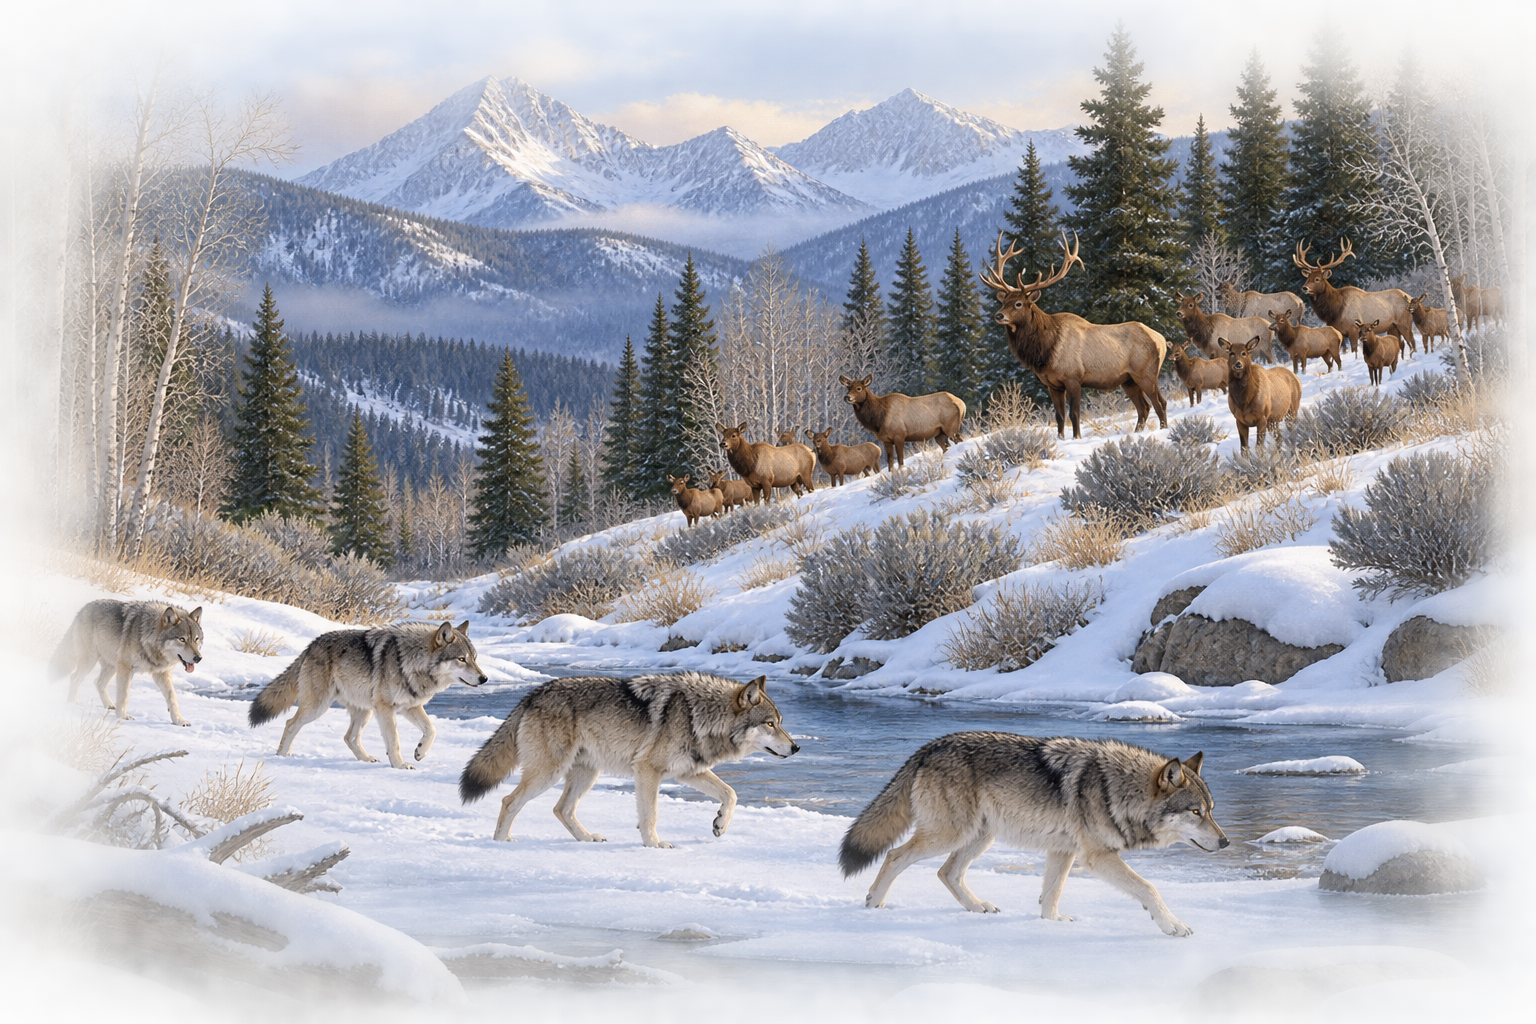
\includegraphics[width=0.6\linewidth]{images/book3/ai/b3-27-wolves-elk.png}

{\small Serigala dan rusa elk di sebuah lembah sungai pada musim
dingin. Pengaruh pemangsanya pada tumbuhannya berjalan lewat tempat
rusa elknya berani merumput sebanyak lewat berapa banyak jumlahnya.}
\end{omfigure}

\begin{method}[Membaca sebuah interaksi dari sebuah percobaan]\label{met:b1:species-interactions:reading}
\begin{enumerate}
  \item Kenalilah manipulasinya (penyingkiran, penambahan, sangkar
        penghalang, pemasangan dalam biakan) dan kendali yang
        dipelihara di sebelahnya pada keadaan yang sama.
  \item Bagi tiap spesiesnya, bandingkan kelimpahannya dengan dan
        tanpa sekutunya: tanda bedanya memberi tanda interaksinya pada
        spesies itu.
  \item Carilah pengaruh tak langsungnya: sebuah spesies yang berubah
        tanpa menyentuh yang dimanipulasinya berada di ujung sebuah
        rantai --- temukanlah perantaranya.
  \item Periksalah skala waktunya (sebuah \omterm{def:b1:species-interactions:types}{persaingan} dapat memakan
        banyak generasi untuk terselesaikan; sebuah riam berjalan pada
        laju aras yang paling lambat) dan skala ruangnya (adakah
        hasilnya berlaku di luar petaknya?).
  \item Paskan modelnya ketika datanya mengizinkan: kurva logistik dan
        \omterm{prop:b1:species-interactions:lotka}{isoklin} bagi \omterm{def:b1:species-interactions:types}{persaingannya}, \omterm{thm:b1:species-interactions:holling}{persamaan cakram} bagi sebuah
        \omterm{def:b1:species-interactions:functional}{tanggapan fungsional}, lalu bacalah parameternya dari gambar
        yang dilinearkan.
\end{enumerate}
\end{method}

\section{Latihan}

\begin{exercise}[$\star$]\label{exo:b1:species-interactions:1}
Berikan pasangan tandanya dan sebuah contoh bagi tiap dari keenam
macam interaksinya.
\end{exercise}

\begin{exercise}[$\star$]\label{exo:b1:species-interactions:2}
Nyatakan asas \omterm{def:b1:species-interactions:competition}{penyisihan bersaing} lalu katakan mengapa ia tidak
melarang lima burung pengicau dalam satu cemara.
\end{exercise}

\begin{exercise}[$\star$]\label{exo:b1:species-interactions:3}
Definisikan \omterm{def:b1:species-interactions:functional}{waktu penanganan} dan laju serangan, lalu berikan laju
makan maksimum seekor pemangsa dengan $h = \qty{30}{min}$.
\end{exercise}

\begin{exercise}[$\star$]\label{exo:b1:species-interactions:4}
Apakah sebuah \omterm{def:b1:species-interactions:keystone}{spesies kunci} itu? Mengapa sebuah \omterm{def:b1:species-interactions:keystone}{spesies kunci} bukan
sekadar yang paling melimpah?
\end{exercise}

\begin{exercise}[$\star\star$]\label{exo:b1:species-interactions:5}
Spesies 1 memiliki $K_1 = 500$, spesies 2 memiliki $K_2 = 400$, dengan $\alpha =
0.5$ dan $\beta = 0.6$. Gambarlah \omterm{prop:b1:species-interactions:lotka}{isoklinnya} lalu berikan hasilnya.
Ulangi dengan $\alpha = 2$, $\beta = 0.6$.
\end{exercise}

\begin{exercise}[$\star\star$]\label{exo:b1:species-interactions:6}
Seekor pemangsa dengan $a = \qty{0.2}{m^2/h}$ dan $h = \qty{0.25}{h}$
berjumpa mangsa pada \qty{10}{} dan \qty{100}{} tiap meter persegi.
Hitunglah laju makannya pada tiap halnya dan kerapatan ketika ia
setengah menjenuh.
\end{exercise}

\begin{exercise}[$\star\star$]\label{exo:b1:species-interactions:7}
Mengapa sebuah tanggapan jenis III memantapkan sebuah \omterm{def:b1:populations:population}{populasi} mangsa
pada kerapatan rendah sedangkan jenis II tidak?
\end{exercise}

\begin{exercise}[$\star\star$]\label{exo:b1:species-interactions:8}
Dari percobaan Gause, jelaskan mengapa \emph{P.~bursaria} berdampingan
dengan \emph{P.~aurelia} tetapi \emph{P.~caudatum} tidak. Apa yang
membuat perbedaannya: laju pertumbuhannya atau \omterm{def:b1:ecosystem-organization:niche}{relungnya}?
\end{exercise}

\begin{exercise}[$\star\star$]\label{exo:b1:species-interactions:9}
Sebuah peniru Batesian menjadi lebih lazim daripada model beracunnya.
Ramalkan apa yang terjadi pada perlindungan keduanya, dan mengapa
keberhasilan penirunya membatasi dirinya sendiri.
\end{exercise}

\begin{exercise}[$\star\star\star$]\label{exo:b1:species-interactions:10}
Petak penyingkiran Paine kehilangan tujuh spesies. Jelaskan, dengan
memakai model \omterm{prop:b1:species-interactions:lotka}{isoklinnya}, bagaimana seekor pemangsa yang memakan
pesaing yang mendominasi mengubah sebuah penyisihan menjadi sebuah
pendampingan.
\end{exercise}

\begin{exercise}[$\star\star\star$]\label{exo:b1:species-interactions:11}
Sebuah jamur \omterm{def:b1:plant-water-minerals:mycorrhiza}{mikoriza} mengambil \qty{15}{\%} fotosintat sebatang
tumbuhan lalu memasok \qty{80}{\%} fosfatnya. Dalam keadaan apa
persekutuannya menjadi sebuah \omterm{def:b1:species-interactions:types}{mutualisme}, dan dalam keadaan apa sebuah
\omterm{def:b1:species-interactions:types}{parasitisme}? Usulkan sebuah percobaan untuk membedakannya.
\end{exercise}

\begin{exercise}[$\star\star\star$]\label{exo:b1:species-interactions:12}
Rancanglah sebuah percobaan untuk menguji apakah serigalanya,
alih-alih cuaca atau perburuannya, menyebabkan pulihnya dedalunya:
kendali, ulangan, peubah yang diukur, dan hasil apa yang akan
menyangkal riamnya.
\end{exercise}

\section{Soal: Pemangsa dan Pantainya}

\begin{problem}[{Soal akhir pekan --- siliata Gause dalam sebuah tabung,
data makan seekor pemangsa yang dipaskan pada persamaan cakram, pantai
Paine dengan dan tanpa bintang lautnya, serta anggaran seekor
penyerbuk, berakhir pada laju serangan dan waktu penanganan
pemangsanya}]
\label{pb:b1:species-interactions:1}

\medskip
\noindent\textbf{Bagian I --- \omterm{def:b1:species-interactions:types}{Persaingan} dalam sebuah tabung.}
Dua siliata ditumbuhkan sendirian: spesies A mencapai $K_A = 200$ tiap
\qty{0.5}{mL} dengan $r_A = \qty{0.8}{d^{-1}}$; spesies B mencapai
$K_B = 130$ dengan $r_B = \qty{0.55}{d^{-1}}$. Bersama, satu individu
B memakai makanan sebanyak $\alpha = 1.4$ individu A, dan satu individu
A sebanyak $\beta = 0.9$ individu B.
\begin{enumerate}
  \item Tuliskan kedua \omterm{prop:b1:species-interactions:lotka}{isoklinnya} dan potongannya pada sumbunya.
  \item Gambarlah keduanya lalu nyatakan spesies mana yang menang, dan
        mengapa hasilnya tidak bergantung pada jumlah awalnya.
  \item Dari waktu lipat duanya ($\ln 2/r$), spesies mana yang akan
        Anda duga menang dari laju pertumbuhannya saja?
  \item Sebuah spesies ketiga C makan di dasar tabungnya lalu bersaing
        dengan A hanya secara lemah ($\alpha = 0.3$, $\beta = 0.3$,
        $K_C = 100$). Gambarlah \omterm{prop:b1:species-interactions:lotka}{isoklinnya} lalu berikan hasilnya.
  \item Mengapa asas penyisihannya berlaku dalam sebuah tabung lalu
        begitu sering gagal dalam sebuah hutan? Berikan dua alasan.
  \item Hitunglah jumlah kesetimbangan A dan C dari perpotongan
        \omterm{prop:b1:species-interactions:lotka}{isoklinnya}.
\end{enumerate}

\medskip
\noindent\textbf{Bagian II --- \omterm{thm:b1:species-interactions:holling}{Persamaan cakramnya}.}
Seekor kumbang pemangsa disuguhi mangsa pada kerapatan 5, 10, 20, 40
dan 80 tiap meter persegi; ia memakan 2,0, 3,3, 5,0, 6,7 dan 8,0
mangsa tiap hari berturut-turut.
\begin{enumerate}[resume]
  \item Gambarkan laju makannya terhadap kerapatannya lalu kenalilah
        jenis tanggapannya.
  \item Hitunglah $1/f$ dan $1/N$ bagi tiap titiknya lalu gambarkan
        keduanya.
  \item Dari kemiringan dan potongannya, perolehlah $a$ dan $h$.
  \item Hitunglah laju makan maksimumnya dan kerapatan setengah
        \omterm{def:b1:lipids:fattyacid}{jenuhnya}.
  \item Pada kerapatan yang mana di antara kelimanya kumbangnya
        membelanjakan lebih dari separuh waktunya untuk menangani?
  \item Mangsa kumbangnya tumbuh secara logistik dengan $r = \qty{0.1}{d^{-1}}$
        dan $K = 200$. Pada kerapatan berapa pertumbuhan mangsanya
        (tiap meter persegi bebas kumbang) setara dengan pemakaian
        kumbangnya bila ada satu kumbang tiap meter persegi? Adakah
        kesetimbangan ini mantap terhadap sebuah kenaikan kecil
        mangsanya?
  \item Sebuah spesies mangsa kedua muncul yang ditangani kumbangnya
        dua kali lebih cepat. Ramalkan perubahan asupan total
        kumbangnya pada kerapatan tinggi.
\end{enumerate}

\medskip
\noindent\textbf{Bagian III --- Pantainya.}
Pada petak kendali Paine \omterm{def:b1:ecosystem-organization:ecosystem}{komunitasnya} memiliki 15 spesies; pada petak
penyingkirannya cacahnya jatuh 15, 12, 10, 9, 8, 8 sepanjang lima
tahun, dan tutupan kerang birunya pada batunya naik dari \qty{20}{\%}
menjadi \qty{85}{\%}.
\begin{enumerate}[resume]
  \item Hitunglah \omterm{def:b1:ecosystem-organization:diversity}{indeks Shannon} sebuah petak dengan 15 spesies pada
        kelimpahan yang setara, dan sebuah petak dengan 8 spesies yang
        kerang birunya \qty{85}{\%} individunya dan ketujuh yang lain
        berbagi sisanya secara merata.
  \item Berapa kali lipat keanekaragamannya jatuh?
  \item Jelaskan, dengan tanda interaksinya, mengapa menyingkirkan
        sebuah interaksi $+/-$ (\omterm{def:b1:species-interactions:types}{pemangsaan} atas kerang birunya)
        menguatkan sebuah interaksi $-/-$ (\omterm{def:b1:species-interactions:types}{persaingan} memperebutkan
        batunya).
  \item Bintang lautnya kurang dari \qty{1}{\%} biomassa petaknya.
        Mengapa biomassa menjadi penuntun yang buruk bagi pentingnya
        sebuah spesies?
  \item Ramalkan apa yang akan terjadi seandainya mangsa pilihan
        bintang lautnya adalah spesies yang paling jarang alih-alih
        yang mendominasi.
  \item Usulkan sebuah cara untuk memastikan bahwa yang bekerja adalah
        \omterm{def:b1:species-interactions:types}{pemangsaan} atas kerang birunya dan bukan sebuah pengaruh lain
        bintang lautnya (sebuah percobaan sangkar).
\end{enumerate}

\medskip
\noindent\textbf{Bagian IV --- Anggaran sebuah \omterm{def:b1:species-interactions:types}{mutualisme}.}
Seekor lebah mengunjungi 1000 bunga dalam sehari lalu mengumpulkan
\qty{40}{mg} gula; tiap bunganya memberikan \qty{40}{\micro g} gula
dalam nektarnya lalu menerima serbuk sari dari, secara purata, 3 bunga
sebelumnya tiap kunjungan. Tumbuhannya membelanjakan \qty{1}{\%}
fotosintat hariannya (\qty{4}{mg} gula tiap bunga) pada nektarnya;
penerbangan seekor lebah memakan biaya \qty{0.5}{mg} gula tiap jam
mencari makan (\qty{8}{h}).
\begin{enumerate}[resume]
  \item Hitunglah perolehan gula harian bersih lebahnya dan setara
        energinya pada \qty{16}{kJ/g}.
  \item Hitunglah biaya harian tumbuhannya tiap bunga sebagai sebuah
        fraksi fotosintatnya lalu katakan apa yang dibelinya.
  \item Mengapa interaksi ini $+/+$ walaupun tiap sekutunya
        mengeksploitasi yang lain?
  \item Seekor perampok nektar menggigit dasar bunganya lalu mengambil
        nektarnya tanpa menyentuh serbuk sarinya. Berikan tanda
        interaksi perampok--tumbuhannya dan pengaruhnya yang mungkin
        pada lebahnya.
  \item Gambarlah diagram tanda tumbuhan, lebah, perampok dan seekor
        burung yang memakan perampoknya, lalu ramalkan pengaruh tak
        langsung burungnya pada tumbuhannya.
  \item Nyatakan hasilnya: laju serangan dan \omterm{def:b1:species-interactions:functional}{waktu penanganan}
        kumbangnya, serta laju makan maksimumnya.
\end{enumerate}
\end{problem}
